\section{Maximum Likelihood and Expectation-Maximization}

\subsection{Maximum Likelihood Equations}
Given Equation \ref{main_pmf}, let the likelihood be
\begin{align*}
L(\mathbb{\theta}) = P(k_1(1), \cdots, k_1(N) | \mathbb{\theta})\ 
\end{align*}
Then, the log-likelihood is
\begin{align*}
\log L(\mathbb{\theta}) &= \sum_{i=1}^{N} \log \left[ \alpha \binom{n}{k_1(i)} p^{k_1(i)} (1-p)^{n - k_1(i)} + (1-\alpha) \binom{n}{k_1(i)} q^{k_1(i)} (1-q)^{n - k_1(i)}  \right] 
\end{align*}

The maximum log-likelihood is given by
\begin{align*}
\hat{\theta} = \argmax_{\theta} \log L(\mathbb{\theta})
\end{align*}

Let $\phi_1$ and $\phi_0$ be functions such that
\begin{align*}
\phi_1(k_1(i)) &= P(k_1(i) | p,n)\\
\phi_0(k_1(i)) &= P(k_1(i) | q,n)
\end{align*}

Therefore, the maximum likelihood equations are given by:
\begin{align*}
\frac{\delta \log P}{\delta \mathbf{\theta}} &= \begin{bmatrix} 
\sum_{i=1}^{N} \frac{\phi_1(k_1(i)) - \phi_0(k_1(i))}{\alpha \phi_1(k_1(i)) + (1-\alpha)\phi_0(k_1(i))} \\ 
\sum_{i=1}^{N} \frac{\alpha \binom{n}{k_1(i)} \left( k_1(i) p^{k_1(i)-1} (1-p)^{n-k_1(i)} - p^{k_1(i)} (n-k_1(i)) (1-p)^{n-k_1(i)-1} \right) }{\alpha \phi_1(k_1(i)) + (1-\alpha)\phi_0(k_1(i))} \\ 
\sum_{i=1}^{N} \frac{(1-\alpha) \binom{n}{k_1(i)} \left( k_1(i) q^{k_1(i)-1} (1-q)^{n-k_1(i)} - q^{k_1(i)} (n-k_1(i)) (1-q)^{n-k_1(i)-1} \right) }{\alpha \phi_1(k_1(i)) + (1-\alpha)\phi_0(k_1(i))} \end{bmatrix} = \mathbf{0}
\end{align*}

\subsection{EM Algorithm}

Let $\mathbf{k_1} = k_1(1), \cdots, k_1(N)$ be the observed data. 
We introduce membership variables $\mathbf{y} = y(i), \cdots, y(N)$ (hidden data) such that $P(y(i) = l) = \alpha_l$. Because we only have two classes, then 
\begin{align*}
P(y(i) = 1) &= \alpha \\
P(y(i) = 0) &= 1-P(y(i) = 1) = 1 - \alpha
\end{align*}

The joint probability mass function is given by:
\begin{align*}
P(\mathbf{k_1}, \mathbf{y} | \theta ) &= \prod_{i=1}^{N} P(k_1(i), y(i) | \theta ) \\
&= \prod_{i=1}^{N} P(k_1(i) | y(i) ) P(y(i) | \theta )  \\
&= \prod_{i=1}^{N} \prod_{l=1}^{M} (\phi_l(k_1(i) \alpha_l)) ^ {I(y(i)=l)}
\end{align*}

Let $Q$ be an auxiliary function such that
\begin{align}
Q(\theta, \theta') &= \mathrm{E} \left[ \log P(\mathbf{k_1}, \mathbf{y} | \theta ) | \mathbf{k_1}, \theta' \right] \nonumber \\
&= \mathrm{E} \left[ \sum_{i=1}^{N} \sum_{l=1}^{M} I(y(i)=l) (\log \phi_l(k_1(i)) + \log \alpha_l) | \mathbf{k_1}, \theta' \right] \nonumber \\
&= \sum_{i=1}^{N} \sum_{l=1}^{M} \mathrm{E} \left[ I(y(i)=l) | \mathbf{k_1}, \theta' \right] (\log \phi_l(k_1(i)) + \log \alpha_l)  \nonumber \\
\label{aux_function}
&= \sum_{i=1}^{N} \sum_{l=1}^{M} P(y(i) = l | k_1(i), \theta') (\log \phi_l(k_1(i)) + \log \alpha_l)
\end{align}

In the E-step of the EM algorithm, we compute the term $P(y(i) = l | k_1(i), \theta')$ of Equation \ref{aux_function}. 
In our case of $M=2$ the E-step is given by:
\begin{align*}
P(y(i) = 1 | k_1(i), \mathbf{\theta'}) &= \frac{\alpha \binom{n}{k_1(i)} p^{k_1(i)} (1-p)^{n-k_1(i)}}{\alpha \binom{n}{k_1(i)} p^{k_1(i)} (1-p)^{n-k_1(i)} + (1-\alpha) \binom{n}{k_1(i)} q^{k_1(i)} (1-q)^{n-k_1(i)}} \\
P(y(i) = 0 | k_1(i), \mathbf{\theta'}) &= \frac{(1-\alpha) \binom{n}{k_1(i)} q^{k_1(i)} (1-q)^{n-k_1(i)}}{\alpha \binom{n}{k_1(i)} p^{k_1(i)} (1-p)^{n-k_1(i)} + (1-\alpha) \binom{n}{k_1(i)} q^{k_1(i)} (1-q)^{n-k_1(i)}}
\end{align*}

In the M-step, we compute
\begin{align*}
\theta^{k+1} &= \argmax_\theta Q(\theta, \theta^{k}) \\
&= \argmax_\theta \sum_{i=1}^{N} \sum_{l=1}^{M} P(y(i) = l | k_1(i), \theta^{k}) (\log \phi_l(k_1(i)) + \log \alpha_l) \\
& \text{s.t. } \sum_{l=1}^{M} \alpha_l = 1
\end{align*}
In our case of $M=2$, we have
\begin{align*}
\theta^{k+1} &= \argmax_\theta \sum_{i=1}^{N} \left[ P(y(i) = 1 | k_1(i), \theta^{k}) (\log \phi_1(k_1(i)) + \log \alpha) + P(y(i) = 0 | k_1(i), \theta^{k}) (\log \phi_0(k_1(i)) + \log (1-\alpha)) \right]
\end{align*}

To maximize $\alpha$, we use a Lagrange multiplier $\lambda$ to define the Lagrangian as
\begin{align*}
L &= \sum_{i=1}^{N} \sum_{l=1}^{M} P(y(i) = l | k_1(i), \theta^{k}) (\log \alpha_l) + \lambda \left( \sum_{l=1}^{M} \alpha_l - 1 \right)
\end{align*}
Then, taking the derivative and making equal to 0:
\begin{align*}
\frac{\delta L}{\delta \alpha_l} &= \sum_{i=1}^{N} P(y(i) = l | k_1(i), \theta^{k})  \frac{1}{\alpha_l} + \lambda = 0 \\
\alpha_l &= -\frac{1}{\lambda} \sum_{i=1}^{N} P(y(i) = l | k_1(i), \theta^{k}) 
\end{align*}
To get the value of the Lagrange multiplier:
\begin{align*}
\frac{\delta L}{\delta \lambda} &= \sum_{l=1}^{M} \alpha_l - 1 = 0 
\end{align*}
Plugging in the value of $\alpha_l$:
\begin{align*}
1 &= \sum_{l=1}^{M} \left[ -\frac{1}{\lambda} \sum_{i=1}^{N} P(y(i) = l | k_1(i), \theta^{k}) \right] \\
1 &=  -\frac{1}{\lambda} \sum_{i=1}^{N} \sum_{l=1}^{M} P(y(i) = l | k_1(i), \theta^{k})\\
\lambda  &= - \sum_{i=1}^{N} \sum_{l=1}^{M} P(y(i) = l | k_1(i), \theta^{k})\\
\lambda  &= - \sum_{i=1}^{N} 1\\
\lambda &= -N
\end{align*}
Therefore, we get:
\begin{align*}
\alpha^{k+1} = \frac{1}{N} \sum_{i=1}^{N} P(y(i) = 1 | k_1(i), \theta^{k})
\end{align*}

To maximize $p$, we get:
\begin{align*}
p^{k+1} &= \argmax_p \sum_{i=1}^{N}  P(y(i) = 1 | k_1(i), \theta^{k}) \log \phi_1(k_1(i)) \\
&= \argmax_p \sum_{i=1}^{N}  P(y(i) = 1 | k_1(i), \theta^{k}) \log \binom{n}{k_1(i)} p^{k_1(i)} (1-p)^{n-k_1(i)}  \\
&= \argmax_p \sum_{i=1}^{N}  P(y(i) = 1 | k_1(i), \theta^{k}) (\log n! - \log k_1(i)! - \log (n-k_1(i))! + k_1(i) \log p + (n-k_1(i)) \log (1-p))
\end{align*}
Taking the derivative and making equal to 0:
\begin{align*}
\frac{\delta}{\delta p} &= \sum_{i=1}^{N}  P(y(i) = 1 | k_1(i), \theta^{k}) \left( \frac{k_1(i)}{p} + \frac{n-k_1(i)}{1-p} \right) \\
&= \sum_{i=1}^{N}  P(y(i) = 1 | k_1(i), \theta^{k}) \left( \frac{k_1(i)(1-p) - (n-k_1(i))p}{p(1-p)}
\right) \\
&= \sum_{i=1}^{N}  P(y(i) = 1 | k_1(i), \theta^{k}) \left( \frac{k_1(i)- k_1(i)p - np +k_1(i)p}{p(1-p)} \right) \\
&= \sum_{i=1}^{N}  P(y(i) = 1 | k_1(i), \theta^{k}) \left( \frac{k_1(i)- np}{p(1-p)} \right) \\
&= \frac{1}{p(1-p)} \sum_{i=1}^{N} P(y(i) = 1 | k_1(i), \theta^{k}) k_1(i) - \frac{1}{p(1-p)} \sum_{i=1}^{N} P(y(i) = 1 | k_1(i), \theta^{k}) np \\
&= 0 \\
\end{align*}
Therefore, the value that maximizes $p$ is
\begin{align*}
p^{k+1} = \frac{\sum_{i=1}^{N} P(y(i) = 1 | k_1(i), \theta^{k}) k_1(i)}{n \sum_{i=1}^{N} P(y(i) = 1 | k_1(i), \theta^{k})}
\end{align*}
To maximize $q$, we take a similar derivation from the one taken for $p$. Therefore, the value that maximizes $q$ is
\begin{align*}
q^{k+1} &= \frac{\sum_{i=1}^{N} P(y(i) = 0 | k_1(i), \theta^{k}) k_1(i)}{n \sum_{i=1}^{N} P(y(i) = 0 | k_1(i), \theta^{k})}
\end{align*}


%Then, we get:
%\begin{align*}
%\alpha_1^{k+1} &= \alpha^{k+1} = \frac{1}{N} \sum_{i=1}^{N} P(y(i) = 1 | k_1(i), \theta^{k}) \\
%\alpha_0^{k+1} &= 1 - \alpha^{k+1} \\
%p^{k+1} &= \frac{\sum_{i=1}^{N} P(y(i) = 1 | k_1(i), \theta^{k}) k_1(i)}{n \sum_{i=1}^{N} P(y(i) = 1 | k_1(i), \theta^{k})} \\
%q^{k+1} &= \frac{\sum_{i=1}^{N} P(y(i) = 0 | k_1(i), \theta^{k}) k_1(i)}{n \sum_{i=1}^{N} P(y(i) = 0 | k_1(i), \theta^{k})}
%\end{align*}


\begin{figure}[!htbp]
	\centering
	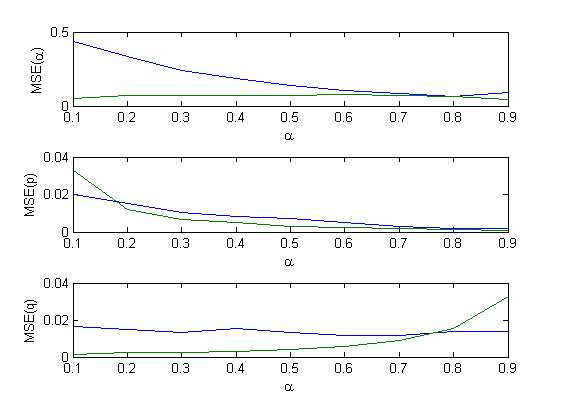
\includegraphics[width=\columnwidth]{images/EM_plot.png} %height=1.7in,
	\vspace{-1pt}
	\caption{CRLB (green) vs EM (blue).}
	\vspace{-2pt}
	\label{figure:crlb-em}
\end{figure}

